%% ============================================================
%% EMRS Spring Meeting Poster
%% "Material Stack Discovery for BEOL-Compatible Quantum
%%  Electronic Nose"
%% Abhineet Agarwal & Swaroop Ganguly, IIT Bombay
%%
%% Compile on Overleaf (pdfLaTeX). Upload this file plus:
%%   fig2_band_diagram.pdf  fig3_flowchart.pdf
%%   fig4_IV.pdf            fig5_d2IdV2.pdf
%%   fig7_deltaD.pdf        fig8_temp_dependence.pdf
%% ============================================================
\documentclass[final]{beamer}

\usepackage[
  size=a0,
  orientation=portrait,
  scale=1.32
]{beamerposter}

\usepackage{amsmath,amssymb}
\usepackage{graphicx}
\usepackage{booktabs}
\usepackage{array}
\usepackage{xcolor}
\usepackage{tikz}
\usepackage[most]{tcolorbox}
\usepackage{ragged2e}
\usepackage{microtype}

\usetikzlibrary{arrows.meta, positioning, calc}

% ── Colour palette ───────────────────────────────────────────
\definecolor{navyblue}{HTML}{1A3A5C}
\definecolor{midblue}{HTML}{2C6FAD}
\definecolor{lightblue}{HTML}{D6E8F7}

\definecolor{orange}{HTML}{C0562A}
\definecolor{lightorange}{HTML}{FAE5D9}
\definecolor{lightgray}{HTML}{F4F4F6}
\definecolor{darkgray}{HTML}{3A3A3A}
\definecolor{forestgreen}{HTML}{2E7D32}
\definecolor{lightgreen}{HTML}{E8F5E9}
\definecolor{rowblue}{HTML}{EBF4FB}

% ── Beamer stripped to blank canvas ─────────────────────────
\usetheme{default}
\setbeamercolor{background canvas}{bg=white}
\setbeamercolor{normal text}{fg=darkgray}
\setbeamertemplate{navigation symbols}{}
\setbeamertemplate{headline}{}
\setbeamertemplate{footline}{}

% ── tcolorbox styles ─────────────────────────────────────────
\tcbset{
  posterbox/.style={
    enhanced, arc=5pt, boxrule=1.2pt,
    colback=lightgray, colframe=navyblue,
    colbacktitle=navyblue, coltitle=white,
    fonttitle=\bfseries\large,
    left=8pt, right=8pt, top=10pt, bottom=12pt,
    toptitle=6pt, bottomtitle=6pt,
  },
  resultbox/.style={
    posterbox,
    colback=lightblue, colframe=midblue,
    colbacktitle=midblue,
  },
  herobox/.style={
    posterbox,
    colback=white, colframe=orange,
    colbacktitle=orange,
  },
  greenbox/.style={
    posterbox,
    colback=lightgreen, colframe=forestgreen,
    colbacktitle=forestgreen,
  },
  methodbox/.style={
    enhanced, arc=4pt, boxrule=0.9pt,
    colback=lightgray, colframe=midblue,
    colbacktitle=midblue, coltitle=white,
    fonttitle=\bfseries\normalsize,
    left=6pt, right=6pt, top=4pt, bottom=6pt,
    toptitle=3pt, bottomtitle=3pt,
  },
  callout/.style={
    enhanced, arc=4pt, boxrule=1.2pt,
    colback=lightorange, colframe=orange,
    left=8pt, right=8pt, top=6pt, bottom=6pt,
    fontupper=\bfseries\small,
  },
}

\setlength{\columnsep}{16pt}

% ============================================================
\begin{document}
\begin{frame}[t]{}
\vspace{-6pt}

%% ── TITLE BAR ───────────────────────────────────────────────
\begin{tcolorbox}[
  enhanced, colback=navyblue, colframe=navyblue,
  arc=0pt, boxrule=0pt,
  left=28pt, right=28pt, top=16pt, bottom=14pt,
]
{\color{white}\bfseries\fontsize{44}{54}\selectfont
  Material Stack Discovery for BEOL-Compatible Quantum Electronic Nose
}\par\vspace{10pt}
{\color{lightblue}
  Abhineet Agarwal \&
  Swaroop Ganguly \\[4pt]
  \normalsize Department of Electrical Engineering,
  Indian Institute of Technology Bombay, Mumbai, India\\
  \texttt{abhineetagarwal@iitb.ac.in}
}\par\vspace{6pt}
{\color{white}\normalsize
  \textit{EMRS Spring Meeting 2026}
}
\end{tcolorbox}

\vspace{10pt}

%% ── THREE-COLUMN BODY ────────────────────────────────────────
\begin{columns}[T]

%% ═══════════════ COLUMN 1 (29%) ═════════════════════════════
\begin{column}{0.290\textwidth}

%% ── MOTIVATION ──────────────────────────────────────────────
\begin{tcolorbox}[posterbox,
  title={Motivation: Room-Temperature IETS}]
\justifying\small

\textbf{IETS} identifies molecules via vibrational fingerprints:
peaks in $d^2I/dV^2$ at bias $V = \hbar\omega/e$ for each
bond-stretching mode.

\vspace{8pt}
\textbf{Fundamental problem.} In conventional metal-insulator-metal
(MIM) junctions, thermal broadening (${\sim}k_BT$) washes out the
peaks below 10\,K (Lambe \& Jaklevic, 1966\,[1]).

\vspace{8pt}
\begin{tcolorbox}[callout]
  RTD solution [2]: the quantum-well resonance acts as an
  energy filter narrower than $k_BT$, restoring
  $d^2I/dV^2$ peaks at \textbf{300\,K}.
\end{tcolorbox}

\vspace{10pt}
\textbf{Remaining gap.} Patil's proof-of-concept [2] used
GaAs/AlAs - grown by MBE at $>700\,^\circ$C, incompatible with
CMOS back-end-of-line (BEOL) processing.

\vspace{8pt}
\textbf{This work.} Systematic literature review and subsequent computational screening of
\textbf{4 oxide heterostructures} (all ALD-depositable below
$400\,^\circ$C) to find BEOL-compatible stacks with
CBO\,$\approx$\,0.5\,eV - the value that brings resonant
tunneling into the molecular vibration window (50–400\,meV).
\end{tcolorbox}

\vfill

%% ── DESIGN RULE ─────────────────────────────────────────────
\begin{tcolorbox}[posterbox,
  title={The Design Rule: CBO $\approx$ 0.5\,eV}]
\centering\small

\resizebox{\linewidth}{!}{%
\begin{tikzpicture}[font=\normalsize]
  % y-axis: V_res (V)
  \draw[->,thick](0,-1.8)--(0,5.6)
    node[above,font=\normalsize]{$V_\mathrm{res}$ (V)};
  \foreach \y/\lab in {1/1,2/2,3/3,4/4,5/5}{
    \draw(-0.14,\y)--(0,\y) node[left,font=\normalsize]{\lab};
  }
  \draw[gray!40,thin](-0.2,0)--(9.4,0);

  % Vibration window band (0.05–0.40 V)
  \fill[forestgreen!22](0,0.05) rectangle (9.4,0.40);
  \draw[forestgreen,dashed,thick](0,0.40)--(9.4,0.40);
  \node[forestgreen!75!black,right,font=\normalsize]
    at (0.15,0.23){Vibration window\enspace 50–400\,mV};

  % High-CBO bars (x-centres 1.5, 3.0, 4.5; width 0.64)
  \fill[red!60](1.18,0) rectangle (1.82,4.3);
  \fill[red!60](2.68,0) rectangle (3.32,3.6);
  \fill[red!60](4.18,0) rectangle (4.82,4.6);
  \node[red!80!black,font=\normalsize\bfseries,align=center]
    at (3.0,5.2){High-CBO oxides (outside window)};

  % Low-CBO bars (x-centres 6.5, 8.2; width 0.64)
  \fill[midblue!80](6.18,0) rectangle (6.82,1.18);
  \fill[midblue!80](7.88,0) rectangle (8.52,0.55);

  % All labels below x-axis, rotated 45° — no overlap possible
  \node[rotate=45,anchor=north east,font=\normalsize]
    at (1.50,-0.15){In$_2$O$_3$/Al$_2$O$_3$};
  \node[rotate=45,anchor=north east,font=\normalsize]
    at (3.00,-0.15){In$_2$O$_3$/HfO$_2$};
  \node[rotate=45,anchor=north east,font=\normalsize]
    at (4.50,-0.15){ZnO/Al$_2$O$_3$};
  \node[rotate=45,anchor=north east,font=\normalsize]
    at (6.50,-0.15){In$_2$O$_3$/$\kappa$-Ga$_2$O$_3$};
  \node[rotate=45,anchor=north east,font=\normalsize\bfseries]
    at (8.20,-0.15){\textbf{ZnO/MgZnO}~$\star$};
\end{tikzpicture}%
}

\vspace{4pt}
\justifying\small
High-CBO oxides resonate at 3–5\,V, far above the molecular
vibration window. Low-CBO stacks with CBO\,$\approx$\,0.5\,eV
bring $V_\mathrm{res}$ into the sensing range.
\end{tcolorbox}

\vfill

%% ── SIMULATION METHOD ───────────────────────────────────────
\begin{tcolorbox}[posterbox, title={Simulation Methodology}]

\begin{tcolorbox}[methodbox,
  title={1.\enspace NEGF + Rank-1 SCBA}]
\small\justifying
For a Gaussian molecular form factor
($\sigma_\mathrm{mol} = 3$\,\AA\,$\ll L_\perp$), the
electron-vibron coupling matrix factorises:
\[
  M = D_0\,\chi(z)\,|u\rangle\langle u|
  \quad \bigl(O(10^{-6})\text{ correction}\bigr)
\]
This rank-1 structure collapses the full 3D SCBA to a
single \textbf{scalar 1D projected equation} -
exact for any transverse grid size.
\end{tcolorbox}

\vspace{5pt}
\begin{tcolorbox}[methodbox,
  title={2.\enspace Anderson Mixing (DIIS)\,[6]}]
\small\justifying
Fixed-point iteration diverges at the NDR voltage.
We store the last $M\!=\!8$ iterate pairs and solve
$\min\|\sum_i\alpha_i r_i\|^2$ at each step.
All 201 bias points converge in \textbf{10–60 iterations};
$|I_L+I_R|/\max|I| < 0.2\%$.
\end{tcolorbox}

\vspace{5pt}
\begin{tcolorbox}[methodbox,
  title={3.\enspace Analytic $d^2I/dV^2$}]
\small\justifying
Numerical double-differencing amplifies SCBA jitter
${\sim}16\times$ near NDR. We evaluate a closed-form
thermal kernel directly from the converged Green's
function - no smoothing needed.
\end{tcolorbox}

\vspace{6pt}
\centering
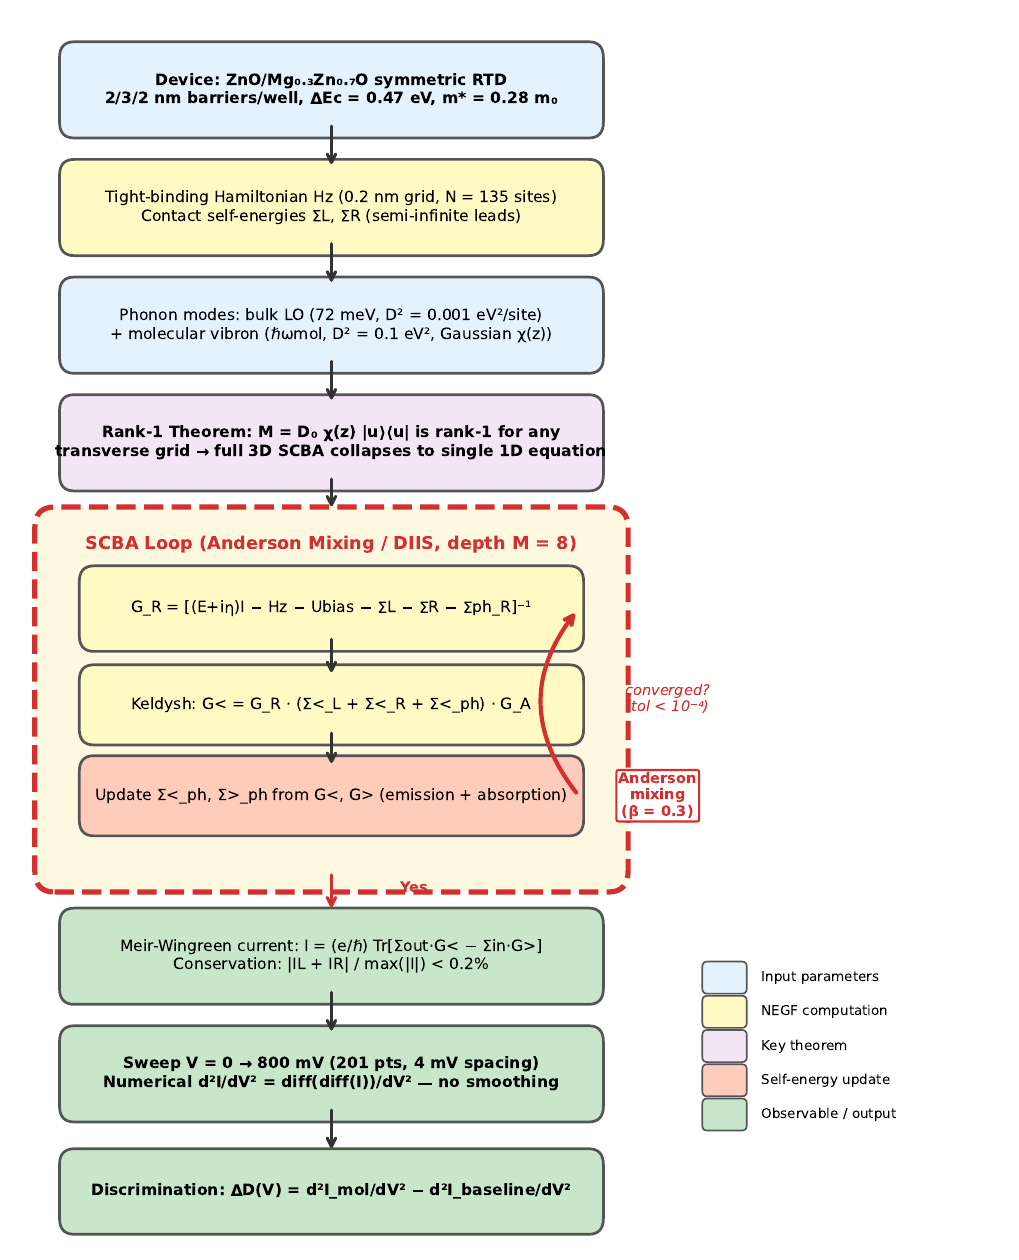
\includegraphics[width=\linewidth]{fig3_flowchart.png}
{\scriptsize \textbf{Fig.\,1.} Rank-1 projected NEGF–SCBA
loop. Molecular coupling is rank-1 for \emph{any} transverse
grid; Anderson mixing (DIIS) ensures convergence.}
\end{tcolorbox}

\end{column}
%% ══════════ end col 1 ════════════════════════════════════════


%% ═══════════════ COLUMN 2 (37%) ═════════════════════════════
\begin{column}{0.370\textwidth}

%% ── MATERIAL TABLE ──────────────────────────────────────────
\begin{tcolorbox}[posterbox,
  title={Material Screening: 12 Oxide Combinations}]
\justifying\small

We screened four well materials (In$_2$O$_3$, IGZO, ZnO,
SnO$_2$) against three barrier classes
(high-CBO: Al$_2$O$_3$, HfO$_2$; low-CBO: Ga$_2$O$_3$
polymorphs, MgZnO alloys). All are ALD-depositable
below 400\,°C.

\vspace{8pt}
\centering
\renewcommand{\arraystretch}{1.3}
\begin{tabular}{@{}lccccr@{}}
\toprule
\textbf{Stack}
  & \textbf{CBO} & \textbf{$m^*/m_0$}
  & \textbf{NDR} & \textbf{BEOL} & \textbf{Ref.}\\
  & (eV) & & & &\\
\midrule
AlGaAs/GaAs
  & 0.23 & 0.067
  & \textcolor{forestgreen}{\textbf{Yes}}
  & \textcolor{red}{No} & [8]\\
GaN/AlN
  & 1.8 & 0.20
  & \textcolor{forestgreen}{\textbf{Yes}}
  & \textcolor{red}{No} & [9]\\
In$_2$O$_3$/$\kappa$-Ga$_2$O$_3$
  & 0.45 & 0.30
  & \textcolor{red}{No}
  & \textcolor{forestgreen}{\textbf{Yes}} & [10,11]\\
%\rowcolor{rowblue}
\textbf{ZnO/Mg$_{0.3}$Zn$_{0.7}$O}
  & \textbf{0.47} & \textbf{0.28}
  & \textcolor{forestgreen}{\textbf{Yes}}
  & \textcolor{forestgreen}{\textbf{Yes}} & [3,4]\\
\bottomrule
\multicolumn{6}{@{}l}{\scriptsize
  $^\ddagger$Ref.\,[3] uses $x\!=\!0.2$; this work uses
  $x\!=\!0.3$ (CBO\,$=1.57x$\,[12]).}
\end{tabular}

\vspace{8pt}
\justifying
\begin{tcolorbox}[callout]
Only ZnO/Mg$_{0.3}$Zn$_{0.7}$O satisfies all three
criteria: CBO\,$\approx\!0.5$\,eV, experimentally
demonstrated NDR, and BEOL-compatible ALD below 350\,°C.
\end{tcolorbox}
\end{tcolorbox}

\vfill

%% ── SELECTED STACK ──────────────────────────────────────────
\begin{tcolorbox}[greenbox,
  title={Selected Stack: ZnO/Mg$_{0.3}$Zn$_{0.7}$O RTD}]
\justifying\small

ZnO/MgZnO uniquely clears all criteria: NDR demonstrated in
experiment [3,4], PVCR\,$\sim$\,6 in simulation, CBO tunable
as $1.57\,x_\mathrm{Mg}$, ALD below 350\,°C, wurtzite
phase-stable at $x_\mathrm{Mg} \leq 0.33$.

\vspace{6pt}
\textbf{Simulated structure:} symmetric 2\,nm MgZnO /
3\,nm ZnO well / 2\,nm MgZnO, with 10\,nm $n^+$-ZnO
contacts ($N_D = 10^{25}$\,m$^{-3}$).
$\Delta E_c = 0.47$\,eV,
$m^* = 0.28\,m_0$,
$\hbar\omega_\mathrm{LO} = 72$\,meV.
Single bound state $E_1 = 149$\,meV.
NDR at $V_\mathrm{res} \approx 552$\,mV (201-pt SCBA,
300\,K); peak current $\sim$72\,nA, PVR\,$\sim$\,6.

\vspace{8pt}
\includegraphics[width=\linewidth]{fig2_band_diagram-2.png}
{\scriptsize \textbf{Fig.\,2.} Conduction-band profile.
(i)\;$V\!=\!0$: bound state $E_1\!=\!149$\,meV; orange
Gaussian $\chi(z)$ marks molecular coupling.
(ii)\;At resonance $V\!\approx\!552$\,mV: $E_1$ aligns
with $\mu_L$, enabling resonant tunneling.
Symmetric bias: $\mu_{L,R}\!=\!E_F \pm V/2$.}
\end{tcolorbox}

\vfill

%% ── IV + d2I ────────────────────────────────────────────────
\begin{tcolorbox}[resultbox, title={I--V and $d^2I/dV^2$ at 300\,K (SCBA)}]

\begin{columns}[T]
  \begin{column}{0.475\linewidth}
    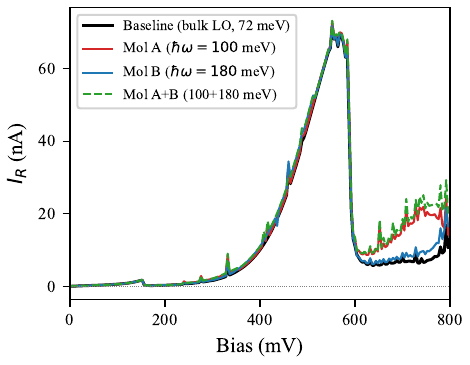
\includegraphics[width=\linewidth]{fig4_IV.png}
    {\scriptsize \textbf{(a)} I–V at 300\,K.
    NDR at $\approx$552\,mV, peak $\sim$72\,nA,
    PVR\,$\sim$\,6. Molecular phonon channels produce
    species-specific $\Delta I$ in the pre-NDR
    region (200–500\,mV).}
  \end{column}
  \begin{column}{0.475\linewidth}
    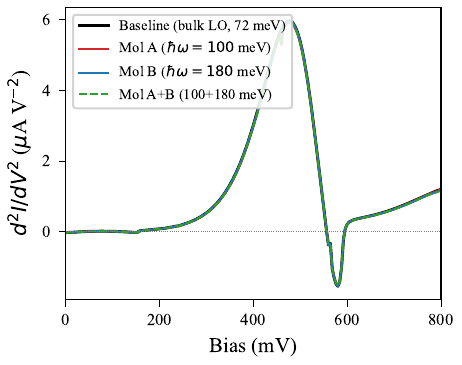
\includegraphics[width=\linewidth]{fig5_d2IdV2.png}
    {\scriptsize \textbf{(b)} $d^2I/dV^2$ at 300\,K.
    Peaks at 100\,mV (Mol\,A) and 180\,mV (Mol\,B)
    correspond to vibrational thresholds
    $V\!=\!\hbar\omega/e$.}
  \end{column}
\end{columns}

\vspace{18pt}
\small Analytes: Mol\,A ($\hbar\omega\!=\!100$\,meV),
Mol\,B ($\hbar\omega\!=\!180$\,meV), Mol\,AB (both).
These synthetic modes sample the odorant fingerprint band
(50–200\,meV) characterised by Pandey et al.\ [7].
201 bias points, 4\,mV spacing.

\end{tcolorbox}

\vfill

%% ── ODORANT COVERAGE ────────────────────────────────────────
\begin{tcolorbox}[posterbox,
  title={Coverage of Real Odorant Vibrational Modes [7]}]
\centering\small
\resizebox{\linewidth}{!}{%
\begin{tikzpicture}[font=\normalsize]
  %% Vertical stacked band diagram
  %% Scale: 1 unit = 200 meV
  %% 50 meV -> 0.25 | 250 -> 1.25 | 400 -> 2.00 | 552 -> 2.76 | 600 -> 3.00

  % Band 1: fingerprint (50–250 meV) — green
  \fill[forestgreen!55](0,0.25) rectangle (5.2,1.25);
  % Band 2: rest of ZnO window (250–552 meV) — blue
  \fill[midblue!65](0,1.25) rectangle (5.2,2.76);
  % Band 3: uncovered (552–600 meV) — gray
  \fill[gray!38](0,2.76) rectangle (5.2,3.00);

  % Outline and internal border
  \draw[darkgray,line width=0.9pt](0,0.25) rectangle (5.2,3.00);
  \draw[darkgray!40](0,1.25)--(5.2,1.25);

  % V_res dashed line at y=2.76 (=552 meV)
  \draw[orange,thick,dashed](-0.5,2.76)--(5.3,2.76);
  \node[orange,font=\normalsize,right] at (5.35,2.76)
    {$V_\mathrm{res}=552$\,mV};

  % Labels inside bands
  \node[forestgreen!20!black,font=\normalsize\bfseries,align=center]
    at (2.6,0.75){Fingerprint band (55\%)\\[2pt]\small 50–250\,meV};
  \node[white,font=\normalsize\bfseries,align=center]
    at (2.6,2.00){ZnO/MgZnO window (76\%)\\[2pt]\small 50–552\,meV};
  \node[darkgray!80,font=\small,align=center]
    at (2.6,2.88){Not covered (24\%)};

  % y-axis (energy axis)
  \draw[->,thick](-0.5,0.10)--(-0.5,3.30)
    node[above,font=\normalsize]{$\hbar\omega$ (meV)};
  % Ticks only at key boundaries (no 200/250 clash)
  \foreach \y/\lab in {0.25/50, 1.25/250, 2.00/400, 2.76/552, 3.00/600}{
    \draw(-0.62,\y)--(-0.50,\y) node[left,font=\normalsize]{\lab};
  }
\end{tikzpicture}%
}

\vspace{2pt}
\justifying\small
The ZnO/MgZnO NDR at 552\,mV covers 76\% of all odorant
modes and the full fingerprint band (50–250\,meV).
\end{tcolorbox}

\end{column}
%% ══════════ end col 2 ════════════════════════════════════════


%% ═══════════════ COLUMN 3 (30%) ═════════════════════════════
\begin{column}{0.300\textwidth}

%% ── HERO RESULT ─────────────────────────────────────────────
\begin{tcolorbox}[herobox,
  title={Key Result: Room-Temperature Discrimination}]

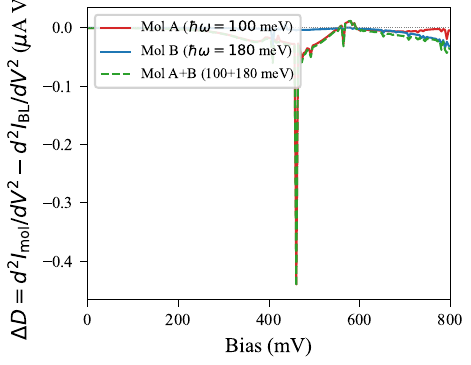
\includegraphics[width=\linewidth]{fig7_deltaD.png}

\vspace{4pt}
{\small
\textbf{Fig.\,3.} Discrimination metric
$\Delta D(V) = d^2I_\mathrm{mol}/dV^2 - d^2I_\mathrm{BL}/dV^2$
at 300\,K. Subtracting the bulk LO-phonon baseline
isolates each molecule's vibrational signature.
}

\vspace{8pt}
\begin{tcolorbox}[callout]
Mol\,A (100\,meV), Mol\,B (180\,meV), and Mol\,AB (both)
produce \textbf{distinct, separable fingerprints at 300\,K
without cryogenic cooling}. Mol\,AB $\approx$ superposition
of A\,+\,B - a consequence of the rank-1 coupling structure.
\end{tcolorbox}
\end{tcolorbox}

\vfill

%% ── TEMPERATURE DEPENDENCE ──────────────────────────────────
\begin{tcolorbox}[resultbox,
  title={Temperature Dependence - Mol\,A ($\hbar\omega\!=\!100$\,meV)}]

\includegraphics[width=\linewidth]{temp.png}

\vspace{2pt}
{\scriptsize \textbf{Fig.\,4.} 10–300\,K sweep.
\textbf{(a)} I–V: peak current rises from $\sim$73\,nA
(300\,K) to $\sim$110\,nA (10\,K) as Fermi smearing
decreases.
\textbf{(b)} $d^2I/dV^2$: IETS peak at 100\,mV sharpens
at low $T$ but remains clearly resolved at 300\,K,
confirming that the RTD resonance preserves vibrational
fingerprints beyond the thermal-broadening limit $3k_BT$.}
\end{tcolorbox}

\vfill

%% ── CONCLUSIONS ─────────────────────────────────────────────
\begin{tcolorbox}[posterbox, title={Conclusions}]
\small
\begin{itemize}\setlength\itemsep{9pt}
  \item[\textcolor{navyblue}{$\blacktriangleright$}]
    High-CBO oxides (e.g.\ In$_2$O$_3$/Al$_2$O$_3$,
    CBO\,=\,2.8\,eV) resonate at 3–5\,V, outside the
    molecular vibration window.
  \item[\textcolor{navyblue}{$\blacktriangleright$}]
    \textbf{Design rule}: CBO\,$\approx$\,0.5\,eV aligns
    $V_\mathrm{res}$ with the 50–400\,meV fingerprint band.
    ZnO/Mg$_{0.3}$Zn$_{0.7}$O is the only oxide pair with
    demonstrated NDR and full BEOL compatibility.
  \item[\textcolor{navyblue}{$\blacktriangleright$}]
    Rank-1 NEGF–SCBA with Anderson mixing achieves
    $<0.2\%$ current conservation across 201 bias points.
  \item[\textcolor{navyblue}{$\blacktriangleright$}]
    Three synthetic odorants \textbf{discriminated at 300\,K}
    via distinct $\Delta D(V)$ patterns - no cryogenics.
  \item[\textcolor{navyblue}{$\blacktriangleright$}]
    NDR at 552\,mV covers \textbf{76\%} of all odorant
    vibrational modes.
\end{itemize}
\end{tcolorbox}

\vfill

%% ── NEXT STEPS ──────────────────────────────────────────────
\begin{tcolorbox}[methodbox, title={Open Items \& Future Work}]
\small
\begin{itemize}\setlength\itemsep{7pt}
  \item Self-consistent Poisson loop
        ($U_\mathrm{bias}$ currently linear-drop; shifts
        $V_\mathrm{NDR}$ by $\sim$5–15\%)
  \item DFT-calibrated Fröhlich coupling
        ($D_\mathrm{bulk}^2$ empirical)
  \item Replace synthetic analytes with real VOC spectra
        from Pandey et al.\ [7]
  \item Fabrication: ALD ZnO/MgZnO RTD on CMOS
        backend test structure
\end{itemize}
\end{tcolorbox}

\vfill

%% ── REFERENCES ──────────────────────────────────────────────
\begin{tcolorbox}[posterbox, title={References}]
{\scriptsize
\begin{enumerate}\setlength\itemsep{1pt}
  \item R.C.\ Jaklevic \& J.\ Lambe, PRL \textbf{17}, 1139 (1966).
  \item A.\ Patil, D.\ Saha, S.\ Ganguly, Sci.\ Rep.\ \textbf{8}, 128 (2018).
  \item S.\ Krishnamoorthy et al., Solid-State Electron.\ \textbf{46}, 1633 (2002).
  \item I.-C.\ Cheng et al., IEEE EDL \textbf{36}, 1330 (2015).
  \item S.\ Datta, \textit{Quantum Transport}, Cambridge (2005).
  \item D.G.\ Anderson, J.\ ACM \textbf{12}, 547 (1965).
  \item N.\ Pandey et al., Sci.\ Rep.\ \textbf{11}, 11389 (2021).
  \item T.C.L.G.\ Sollner et al., APL \textbf{43}, 588 (1983).
  \item C.\ Bayram et al., APL \textbf{96}, 042103 (2010).
  \item Y.\ Kuang et al., ACS AEM \textbf{3}, 795 (2021).
  \item J.\ Zhu et al., Nanotechnology \textbf{35}, no.\,43 (2024).
  \item H.\ Yin et al., Sci.\ Rep.\ \textbf{7}, 41567 (2017).
\end{enumerate}
}
\end{tcolorbox}

\end{column}
%% ══════════ end col 3 ════════════════════════════════════════

\end{columns}

\end{frame}
\end{document}
